\chapterimage{head2.png} % Chapter heading image
\chapter{Langevin Dynamics}
\section{Basic Equation}
\begin{definition}
\begin{align}
        dx_t=D F(x_t)dt  + \sqrt{2D}d{W}_t.
\end{align}
\label{langevin}
\end{definition}

\subsection{The most disordered dynamics as reference}
\begin{align}
      V_{\rm ref}(x) &= 0\\
      F_{\rm ref}(x) &= 0\\
      D &= 4.845 \times 10^{9}~~\text{\AA}^2~s^{-1}  
\end{align}

\begin{center}
        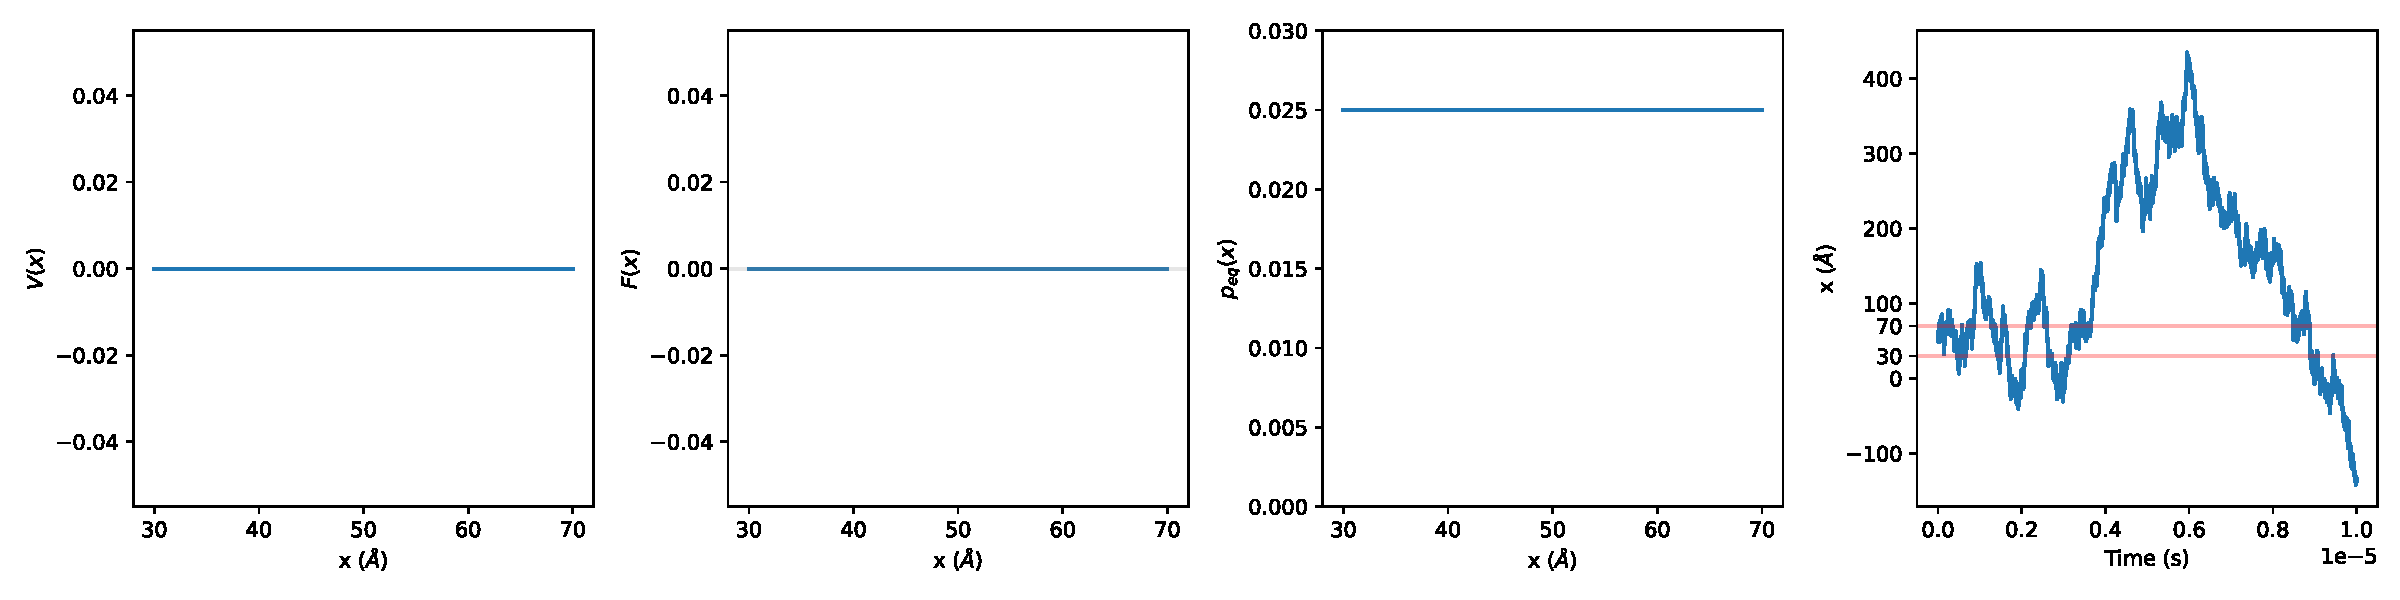
\includegraphics[scale=0.35]{ch1/zero_force_dynamic.pdf} 
\end{center}

\subsection{Harmonic Well}
\begin{align}
        V(x) &= k (x-50)^2\\
        F(x) &= 2k(x-50)  \\
        p_{\rm eq}(x) &= \exp{(-V(x))} \\
        D &= 4.845 \times 10^{9}~~\text{\AA}^2~s^{-1}
\end{align}
Here, $k=0.5$ kcal/mol/Å$^2$
\begin{center}
        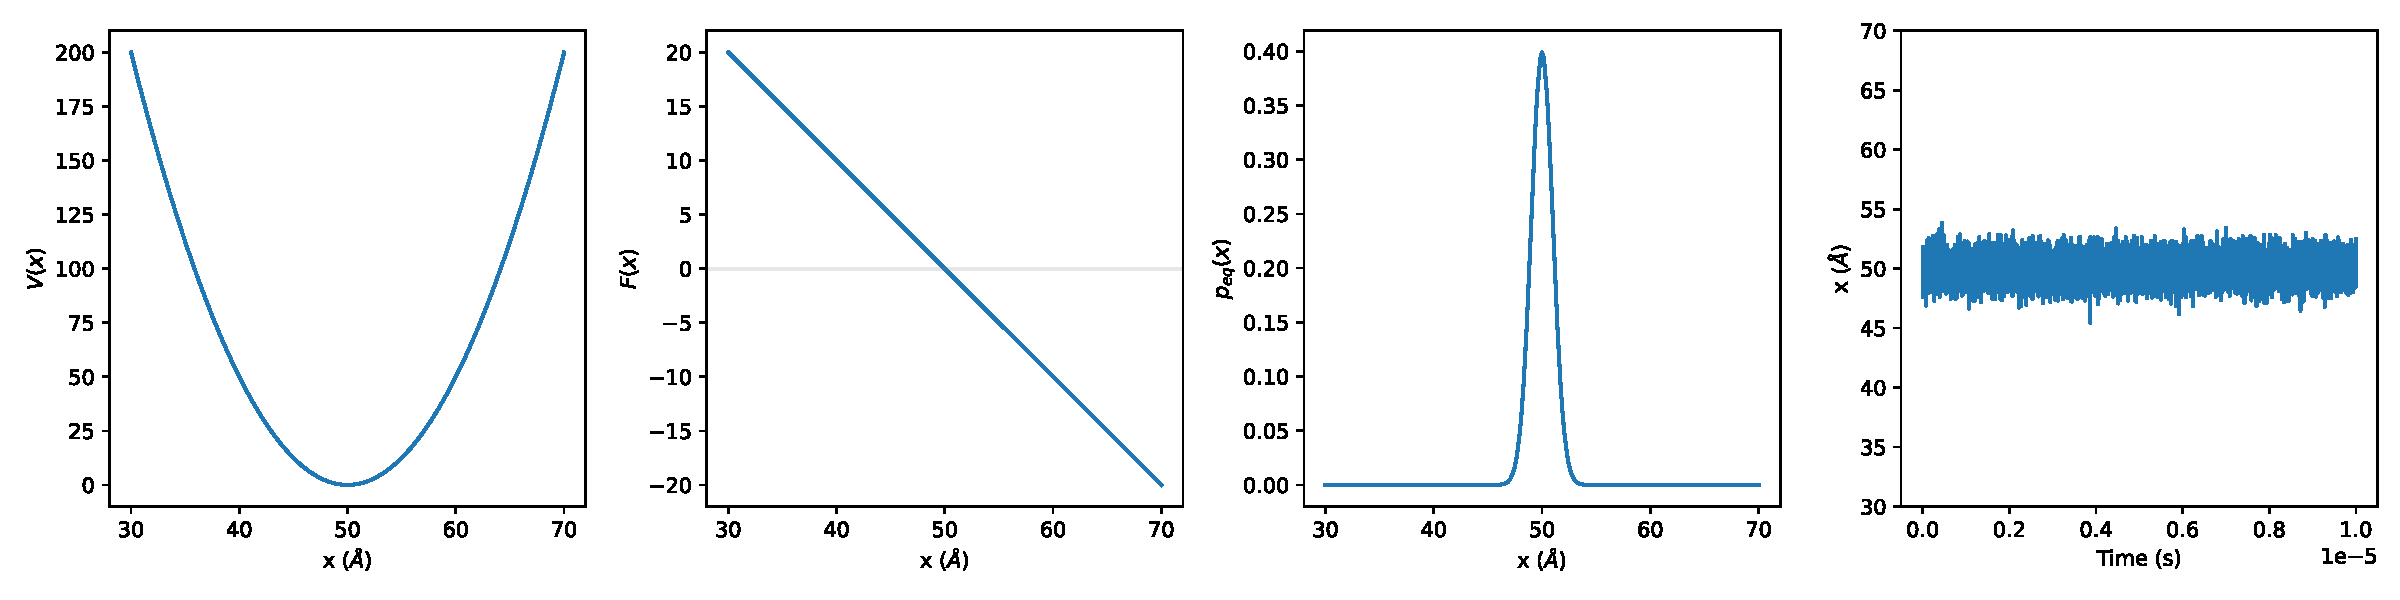
\includegraphics[scale=0.35]{ch1/single_well.pdf} 
\end{center}

\subsection{Double Well}
\begin{align}
        V(x) &= -\frac{1}{4} h^4 x^2 + \frac{1}{2} c^2 x^4 + d\\
        c    &= \sqrt{\frac{2H}{W^4}},H > 0 \\
        h    &= \sqrt{2Wc} \\
        F(x) &= \frac{1}{2} h^4 x - 2 c^2 x^3\\
        p_{\rm eq}(x) &= \exp{(-V(x))} \\
        D &= 4.845 \times 10^{9}~~\text{\AA}^2~s^{-1}\\
\end{align}
where $d$ is y-intercept, $H$ is the height of the central peak, and $W$ is the width between two valleys. In the following case, $H=5$ and $W=10$.
\begin{center}
        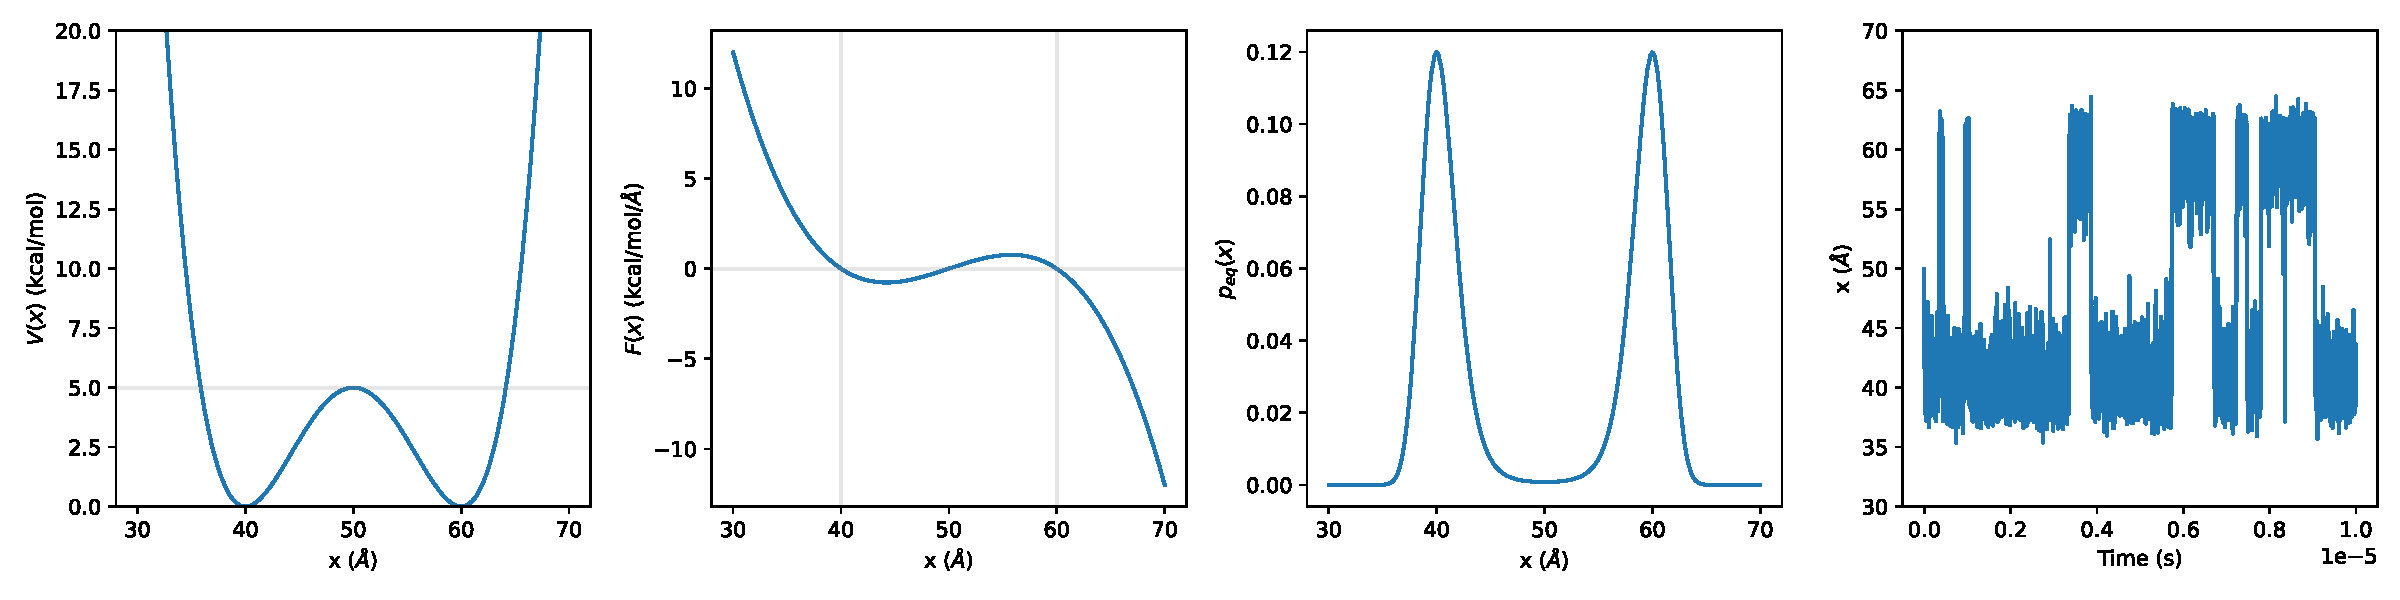
\includegraphics[scale=0.35]{ch1/double_well.pdf} 
\end{center}